\chapter{Ausarbeitung des Architekturkonzepts}\label{chap:concept}
\section{Analyse und Übersetzung der bisherigen UI-Struktur}\label{sec:ui_structure_translation}
Momentan werden alle für die Darstellung der verschiedenen Ansichten benötigten Parameter und Metadaten in einzelnen Dateien als Teil des Solution-Verzeichnis gespeichert. <Ansichtsname>.dli enthält die Konfiguration für die Detailansicht und <Ansichtsname>.vlc die Konfiguration der Übersichtsliste. Für den Aufbau dieser Dateien existiert leider keine offizielle Spezifikation und auch keine Dokumentation, es ist daher eine Herausforderung direkt alle nötigen Informationen aus ihnen auszulesen und bedarf unter Umständen spätere Anpassungen am Auslesetool oder der künftigen Struktur.

\subsection{DLI}
\subsection{VLC}
\subsection{Neue Struktur}
Der Aufbau der neuen Struktur entspricht simplen JSON-Daten. 
% wird auf dem server gespeichert und dient dann direkt auch als langzeitspeicher für die UI (kann in DB serialisiert werden, Änderungen nur auf Clientseite)
% enthält position im grid, anfangs durchnummeriert, später mit von user gesetzten werten

\section{Client}
% react skelett mit komponenten wird ausgeliefert -> aufbau ui dann dynamisch
% ablaufdiagram? client besteht aus App, Detail und Listview, fragt struktur an -> rendert placeholder mit korrekter struktur -> fragt parallel daten an -> zeigt daten an
% bei eigenen änderungen -> daten an server schicken -> server sendet veränderte daten (-> prüfen ob korrekt?)
% bei fremden änderungen -> daten neu rendern

\subsection{React-Komponenten}
Die jetzige Oberfläche besteht aus einer festen Anzahl von Darstellungs-Elementen welche je nach Kontext andere Inhalte anzeigen. Zu den Elementen gehören unter anderem statische Texte, Eingabefelder, Check- und Comboboxen, Gruppierungen und Container für weitere Elemente. Der Kontext für den Inhalt ergibt sich aus dem Datenbankfeld das mit dem jeweiligen Element verknüpft ist und Einstellungen wie Sichtbarkeitsbedingungen oder Formatierungen. Da bereits im Voraus bekannt ist, welche Art von UI-Elementen benötigt werden, können diese auch schon im Vorfeld erstellt werden. Diese fertigen \nameformat{React}-Komponenten werden mit dem Produkt ausgeliefert und können zur Laufzeit dynamisch auf der Webseite platziert werden. Die Funktionalität dieser Elemente orientiert sich dabei immer an der Funktionalität der Originalkomponente.
% props auflisten (evtl. nur gemeinsame?)

\subsection{Komponenten-Layout}
% => nicht nur Elemente sondern auch Anordnung wichtig!!
Für die sinnvolle Nutzung der vorgefertigten Komponenten ist es notwendig, diese nicht nur einfach nacheinander auf der Seite zu platzieren, sondern ein bedienbares Layout für die Platzierung anzubieten. Die Umsetzung wird in diesem Abschnitt dargelegt.

\subsubsection{Erste Überlegungen}
Zu Beginn erschien die zentrale Frage, wie es technisch möglich ist, die Komponenten der Detailansicht vom Benutzer anpassbar anzuordnen. Eine naive Herangehensweise kann in Abbildung~\ref{fig:layout_grid_test} gesehen werden. Umgesetzt wurde dies mit einem CSS-Grid (rote Umrandung) das entweder horizontal oder vertikal in zwei Hälften getrennt werden kann. Jede dieser Hälften stellt abermals ein CSS-Grid dar das beliebig zwischen Elterncontainern verschoben werden kann. Abstrakt handelt es sich bei diesem Ansatz um einen nicht balancierten binären Baum an dessen Endpunkten (Blätter) sich genau eine UI-Komponente (blaue Umrandung) befindet. Es wurde schnell klar dass diese Lösung in ihrer binären Form nicht flexibel genug ist um vorhandene Layouts abzubilden. Da ein Ausbau auf eine Struktur mit variabler Anzahl an Verzweigungen sehr komplex und zeitaufwändig gewesen wäre wurde der Ansatz gänzlich verworfen und nach einer Alternativen Lösung gesucht. \fixme{bessere erklärung und begründung warum nicht flexibel genug}

\begin{figure}
    \centering
    \captionsetup{justification=centering}
    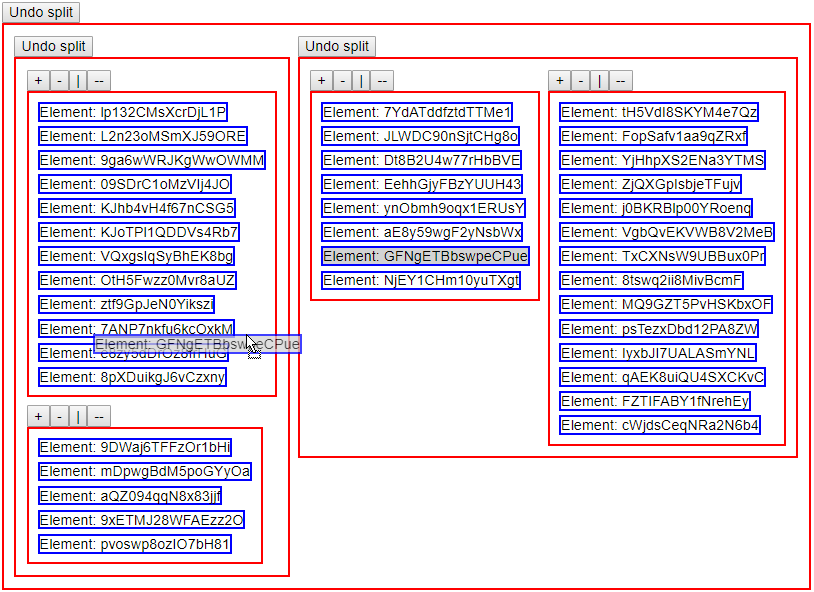
\includegraphics[width=\textwidth]{figures/layout_grid_test.png}
        \caption{Eigener Layout-Prototyp mit CSS-Grids}\label{fig:layout_grid_test}
\end{figure}

\subsubsection{Umsetzung}\label{subsec:layout}
% table / grid

\subsection{Identifikation auf Server}
Um die UI-Elemente mit Daten aus der Datenbank zu befüllen muss eine entsprechende Identifikation möglich sein. Es wird vorausgesetzt dass diese eindeutige ID, ob sie aus Tabellennamen plus Spaltenname der Datenbank oder aus anderen Informationen besteht, zum Zeitpunkt der Übersetzung einer Ansicht bereits bekannt ist und mit ausgelesen werden kann. Bei Anfragen an den Server werden alle IDs der beteiligten Elemente mit an den Server übertragen, ebenso wie dieser bei Antworten immer die IDs der Elemente, für welche die Antwortdaten gedacht sind, sendet.

\subsection{Visualisierung von Lade- und Fehlerzustände}\label{subsec:loading_state_section}
Direktes Feedback ist für die subjektive Einschätzung einer performanten Webseite essentiell. Typischerweise ist die am längsten dauernde Aktion auf einer Webseite das Nachladen von Daten, es ist also sinnvoll diesen Vorgang für Nutzer visuell ansprechend deutlich zu machen. Für diesen Zweck sollen alle React-Komponenten eine visuell simplere Repräsentation von sich selbst in Form von unspezifischen grauen Boxen enthalten, welche nur auf die ungefähre Form und Darstellung mit Echtdaten hindeutet und die bereits während des Ladevorgangs angezeigt werden kann. In Abbildung~\ref{fig:comp_loading_final_comparison} sieht man eine Gegenüberstellung der beiden Repräsentationen (finaler Zustand links, Ladezustand rechts), jeweils für ein Edit-Element und ein Checkbox-Element.

\begin{figure}
    \centering
    \captionsetup{justification=centering}
    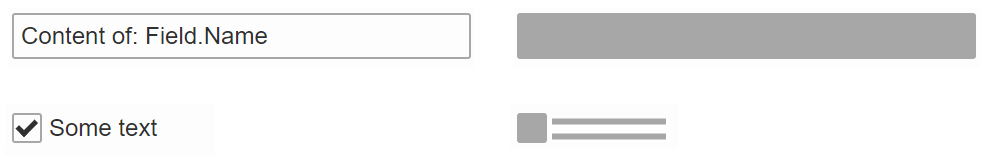
\includegraphics[width=\textwidth]{figures/comp_loading_final_comparison.png}
        \caption{Ladezustand einer Komponente}\label{fig:comp_loading_final_comparison}
\end{figure}

Mit einer entsprechende Einfärbung und einem Hinweistext kann diese Visualisierung, wie in Abbildung~\ref{fig:comp_possible_error_state} an zwei unterschiedlichen Ausführungen gezeigt, ebenfalls dazu genutzt werden um Fehlerzustände beim Laden von Daten zu signalisieren.

\begin{figure}
    \centering
    \captionsetup{justification=centering}
    
\includegraphics[width=\textwidth]{figures/comp_possible_error_state.png}
        \caption{Mögliche Fehlerzustände einer Komponente}\label{fig:comp_possible_error_state}
\end{figure}

\subsection{Einbindung von GraphQL mit Apollo}
% integration erklären: queries so weit wie möglich trennen und zu jeder Komponente speichern

\subsection{Editier-Modus}
% immer.js

\subsection{Individualisierung}
Die Serialisierung des Layouts nach JSON geschieht über die jeweilige Darstellungsbibliothek der Ansicht. Zusätzliche (eigene) Formatierungen aus der Detailansicht werden anschließend im JSON ergänzt und dann auf den Server übertragen. Bevor das erste Mal eine solche Anpassung der Ansichten vorgenommen wird entspricht die Darstellung dabei der in Abschnitt~\ref{sec:ui_structure_translation} beschriebenen, aus der Desktop-UI automatisch generierten Struktur. Das Backend kann diese Informationen entweder direkt als Datei oder in einer NoSQL-Datenbank als Dokument abspeichern, oder seinerseits eine Serialisierung in bestehende SQL-Datenbankschemas vornehmen. Zur Darstellung werden diese Informationen wie in Abschnitt~\ref{subsec:grapql_schema} dargestellt wieder vom Server abgerufen.
% layout und aussehen -> auf server serialisieren

\subsection{Suche, Filter, Sortierung}
Die Darstellung der Übersichtsliste wird, wie oben beschrieben, die \nameformat{React}-Bibliothek \nameformat{\fixme{name aus layout section oben}} (siehe Abschnitt~\ref{subsec:layout}) benutzt. Diese ermöglicht das Suchen, Filtern und Sortieren bereits ohne weitere Anpassungen. Für die Detailansicht müssen im jetzigen Stand analog zum Desktopclient die vorhandenen Möglichkeiten im Backend zur Umsetzung der Suche und Filter genutzt werden. Ein Nachteil dieses Ansatz ist natürlich, dass jedes Mal eine Anfrage an den Server geschickt werden und alle (gefilterten) Daten neu übertragen werden müssen. Eine bessere Alternative bestünde darin, die Daten der Detailansicht ebenfalls durch \nameformat{\fixme{name aus layout section oben}} verarbeiten zu lassen --- die technische Umsetzbarkeit bedarf weiterer Analysen der Bibliothek.

\subsection{Tests und Continuous Integration}


\section{API}
\fixme{more infos?}

\subsection{Aufbau / GraphQL-Schema}\label{subsec:grapql_schema}
Das Schema, welches den Aufbau der Anfragen und damit gleichzeitig der Antworten vorgibt, enthält zwei Einstiegspunkte. Zum einen können Informationen zur Übersichtsliste und zum Anderen die der Detailansicht abgefragt werden. Beide Zweige sind weiterhin in eine Struktur- und einen Datenabschnitt getrennt. Clients können so zuerst die Struktur, also alle Enthaltenen UI-Elemente und deren Platzierung, Formatierung, etc., der Ansicht abfragen. Die reine Struktur enthält im Vergleich wenige Daten, eine entsprechende Abfrage erhält also zügig eine Antwort. Während die UI anschließend anhand der Struktur aufgebaut wird und Lade-Platzhalter (siehe Abschnitt~\ref{subsec:loading_state_section}) anzeigt können parallel die Daten nachgeladen werden. Sobald auch dieser Vorgang abgeschlossen ist werden die Lade-Platzhalter je nach Erfolg beziehungsweise Misserfolg mit den tatsächlichen Feldinhalten oder der Fehlervisualisierung inklusive Fehlermeldung ausgetauscht.

\subsection{Keine Business Logik im Client}
Clients sollten keine eigenen Schlussfolgerungen aus den von der API gelieferten Daten ziehen müssen. Dies ist ein häufig begangener Fehler, bei dem die API Daten zu einer Ressource angibt, diese Daten aber nicht direkt angezeigt sondern erst noch auf irgendeine Art verarbeitet und transformiert werden müssen. Es kann vorkommen, dass verschiedene Implementierungen von Clients an dieser Stelle andere Transformationen anwenden und die sichtbare Darstellung dabei für Endanwender inkonsistent erscheint. Selbst wenn darauf geachtet wird, dass zu einem Zeitpunkt X alle Clients konsistent implementiert sind ist es möglich diese Konsistenz durch Bugfixes oder andere clientspezifische Anpassungen in der Zukunft zu einem beliebigen Zeitpunkt Y wieder zu verlieren. Ein Beispiel für einen solchen Fall, beschrieben von Phil Sturgeon \parencite{sturgeon_2017}, ist eine API die Anfragen über Rechnungen beantwortet und dabei verschiedene Felder liefert. Enthält das Feld `\textbf{bezahlt-am}' keine Daten, können Clients davon ausgehen dass die Rechnung noch nicht bezahlt wurde. Wenn nun ein weiteres Feld, welches anzeigt ob der Betrag tatsächlich auf dem Empfängerkonto eingegangen ist, `\textbf{bezahlung-erhalten-am}' hinzugefügt wird, zeigen alte Clients den Status weiterhin als `Bezahlt', sobald das erste Feld einen Wert enthält. Clients die ein Update erhalten haben zeigen dieses Status jedoch erst, wenn beide Felder einen Wert enthalten.
Entsprechend ist diese API so konzipiert, dass notwendige Transformationen immer im Backend vollzogen werden. In der aktuellen Implementierung gibt es noch keine Instanz bei der dieses Paradigma angewendet werden muss, spätere Anpassungen und Ergänzungen an der API müssen aber entsprechend umgesetzt werden.

